\documentclass[12pt]{report}
\usepackage{graphicx}
\usepackage{fontspec}
\usepackage[utf8]{inputenc}
\usepackage[acronym, nonumberlist, section]{glossaries}
\usepackage[english]{babel}
\usepackage{indentfirst}
\usepackage{titlesec}
\usepackage{float}
\usepackage{tocloft}
\usepackage{titletoc}
\usepackage{etoolbox}
\usepackage{geometry}
\usepackage{etoolbox} % for removing lof, lot grouping

\usepackage[
    backend=biber,
    style=ieee,
  ]{biblatex}
\usepackage{setspace}

%================ SETUP: ACRONYMS
\makeglossaries
\newacronym{bit}{BIT}{Bachelor of Information Technology}
\newacronym{ucsc}{UCSC}{University of Colombo School of Computing}
\newacronym{it}{IT}{Information Technology}
\newacronym{grn}{GRN}{Goods Received Note}
\newacronym{sdlc}{SDLC}{Software Development Life Cycle}
\newacronym{mvc}{MVC}{Model View Controller}
\newacronym{uml}{UML}{Unified Modeling Language}

%================ SETUP: PATHS
\graphicspath{ {./images/} }
\addbibresource{./references/biblography.bib}

%================ SETUP: FORMAT CHAPTER NAMES IN THE DOCUMENT BODY
\titleformat{\chapter}[hang] 
{\normalfont\huge\bfseries}{\chaptertitlename\ \thechapter:}{5pt}{} 
\titlespacing*{\chapter}{0pt}{-30pt}{10pt}


% SETUP: REMOVE CHAPTER GROUPING IN LIST OF TABLES AND LIST OF FIGURES
\makeatletter
\patchcmd{\@chapter}{\addtocontents{lof}{\protect\addvspace{10\p@}}}{}{}{}% LoF
\patchcmd{\@chapter}{\addtocontents{lot}{\protect\addvspace{10\p@}}}{}{}{}% LoT
\makeatother

% ================ SETUP: TABLE OF CONTENTS

% space before and after toc title
\setlength{\cftbeforetoctitleskip}{3pt}
\setlength{\cftaftertoctitleskip}{10pt}

% format chapter titles for ucsc modal
\titlecontents{chapter}
   [0pt]% <left>
   {\addvspace{10pt}}% {above}
%    {\bfseries}% <above-code>
   {\bf\chaptername\ \thecontentslabel:\quad}% <numbered-entry-format>
   {}% <numberless-entry-format>
   {\titlerule*[0.8pc]{.}\contentspage}

% section and sub section spacing
\setlength{\cftbeforesecskip}{10pt}
\setlength{\cftbeforesubsecskip}{10pt}


% dotted lines for chapters
\renewcommand{\cftchapleader}{\cftdotfill{\cftdotsep}}

% ================ SETUP: LIST OF FIGURES
% space before and after lof title
\setlength{\cftbeforeloftitleskip}{3pt}
\setlength{\cftafterloftitleskip}{10pt}

% space before each entry
\setlength{\cftbeforefigskip}{10pt}

% left indent
\setlength{\cftfigindent}{0pt}

% ================ SETUP: LIST OF TABLES
% space before and after lof title
\setlength{\cftbeforelottitleskip}{3pt}
\setlength{\cftafterlottitleskip}{10pt}

% space before each entry
\setlength{\cftbeforetabskip}{10pt}

% left indent
\setlength{\cfttabindent}{0pt}

% ================ SETUP: LIST OF ACRONYMS
\setglossarystyle{tree}

%================ SETUP: FONTS
\setmainfont[
	Path = ./fonts/,
 	BoldFont={LiberationSerif-Bold.ttf}, 
 	ItalicFont={LiberationSerif-Italic.ttf},
 	BoldItalicFont={LiberationSerif-BoldItalic.ttf}
 ]{LiberationSerif-Regular.ttf}
 
%=============== SETUP: MARGIN AND PAGE SETUP
\geometry{a4paper, left=37mm,  top=25mm, bottom=25mm, right=25mm}
% \usepackage[document]{ragged2e} % left-alignment
% \hyphenpenalty=10000
% \tolerance=10000

%--------------------------------
\begin{document}
\onehalfspacing

%=============== SETUP: PARAGRAPH STYLES
\setlength{\parindent}{3em} % start indentation
\setlength{\parskip}{1em} % space between two parapgrahs

%========= PAGE: TITLE PAGE (COVER)
\thispagestyle{empty}
\begin{titlepage}
	\begin{center}
		\vspace*{2cm}
		
\includegraphics[width=0.15\textwidth]{uoc/uoc_logo.jpg}\\
		\vspace{1cm}
		{\LARGE Sales and Production Management System for \\Two Elephants Fireworks}
		\vspace{2cm}
		\begin{large}

			\textbf{D.A.N.P. DISSANAYAKE}\\
			\vspace{2cm}
			BIT Registration Number: R181344 \\
			Index Number: 1813447 \\
			Name of the Client :  Onelli Traders / Two Elephants Fireworks \\
			Name of the supervisor :  J.A. Manjula Sanjeewa \\

			\vspace{1cm}

			\bf{2020/ August}

			\vspace{2.5cm}

			\vfill


			
\includegraphics[width=0.15\textwidth]{uoc/ucsc_logo.png}%
			\begin{minipage}[b]{0.7\textwidth}
				\centering
				{\small \bf Degree of Bachelor of Information Technology of the University of Colombo School of Computing}
			\end{minipage}%
			\includegraphics[width=0.15\textwidth]{uoc/bit_logo.png}
		\end{large}
	\end{center}
\end{titlepage}

%========= PAGE: ABSTRACT
\newpage
\thispagestyle{plain}
\pagenumbering{roman}
\setcounter{page}{2}
\chapter*{\Huge Abstract}
\addcontentsline{toc}{chapter}{\bf{Abstract}}

Two Elephants Fireworks is a gun powder based product manufacturing company based on Walpala. Their products range from
firecrackers to high-power fireworks for large scale events. As a result of that, currently employees of this company has to deal with manually maintaining list of transactions, products and material details. There is no process to store and keep track of customer details at the moment and generating reports to make business decisions and observe growth and customer demands is really hard due to the nature of these manual processes.

Since the current system is manual, it’s very difficult to manage daily sales, orders, material details, billing process and the rest of their daily operations. Having to maintain and keep track of hundreds of books and papers makes it very hard and time consuming to fulfill customer orders and causes some customers to wait for a long period of time. Also, since manually keeping tack of the inventory is needed, it consume lot of manpower and time. Furthermore, due to human errors there are considerable amount of late order  deliveries. The owner of this company is also having trouble checking latest order and sales information while he is traveling.

Taking above issues into consideration, the proposed system  is being developed for a web-based environment. It aims to make it easy to manage daily orders, inventory, material processing, customer details..etc. This system supports users, privileges and accurate report generating for making business decisions. Not only that, but also this will facilitate remote access to the system making it possible to check recent information without having to come to the office.

Visual Studio code was used to implement the proposed system in TypeScript and JavaScript. MySQL and TypeORM is being used to manage the data storing and retrieving aspect of the system. Chart.js and Datatables are used for the report generating process. Furthermore, \acrlong{uml} was used for the analysis and design of the system. Also, this system uses the \acrshort{mvc} architecture and iterative and incremental approach.

This proposed system will achieve client's functional and non-functional requirements by providing an efficient and user friendly environment. Also, this will provide tools to optimize business processes and make decisions based on more accurate reports and data.

%========== PAGE: TABLE OF CONTENT
\newpage
\addcontentsline{toc}{chapter}{\bf{Contents}}
\begin{singlespacing}
	\tableofcontents
\end{singlespacing}
\setlength{\parskip}{1em}
\renewcommand{\baselinestretch}{2.0}

%========== PAGE: LIST OF FIGURES
\newpage
\addcontentsline{toc}{chapter}{\bf{List of Figures}}
\begin{singlespacing}
	\listoffigures
\end{singlespacing}
% \setlength{\parskip}{1em}
\renewcommand{\baselinestretch}{2.0}

%========== PAGE: LIST OF TABLES
\newpage
\addcontentsline{toc}{chapter}{\bf{List of Tables}}
\begin{singlespacing}
	\listoftables
\end{singlespacing}
% \setlength{\parskip}{1em}
\renewcommand{\baselinestretch}{2.0}

%========== PAGE: LIST OF ACRONYMS
% \section*{\Huge List of Acronyms}
% \addcontentsline{toc}{chapter}{\bf{List of Acronyms}}
\newpage
\addcontentsline{toc}{chapter}{\bf{List of Acronyms}}
\printglossary[type=\acronymtype,title=\Huge{List of Acronyms}]

% \setlength{\parskip}{1em}
% \renewcommand{\baselinestretch}{2.0}

%================ SETUP: SECTION TITLE FONT SIZES
\titleformat*{\section}{\fontsize{16}{19}\bfseries\normalfont}
\titleformat*{\subsection}{\fontsize{14}{17}\bfseries\normalfont}
\titleformat*{\subsubsection}{\fontsize{12}{15}\bfseries\normalfont}

%>>>>>>>>>>>>>>>>>>>>>>>>>>>>>>>>>>>>>>>>
% Main body of Thesis
%========= Start of Thesis 
\newpage
\pagenumbering{arabic}
\setcounter{page}{1}
\onehalfspacing

\chapter{Introduction}
This chapter introduces background information of the selected company for the project, the problem going to be solved, objectives hoping to accomplish and scope of the project.

\section{Motivation for the project}
Two Elephants Fireworks is one of the major gun powder based product manufacturers in  the Andiambalama. But currently all of their processes and paperwork are done manually. Due to high number of clients and suppliers, managing all of their operations manually has become a very time consuming inefficient task. Below are some of the difficulties they have to face because of their current way of performing tasks.

\begin{itemize}
	\item There is no proper way to manage customer details so they have to request same details over and over again.
	\item Customer order management process is very time consuming and inconsistent.
	\item They are unable to properly calculate measurements of raw materials needed to complete an order.
	\item Lot of materials and processed materials go to waste because there is no way to properly keep track of the inventory.
	\item There is no way to generate reports about sales and inventory to make business decisions such as when to increase the production \& supply.
	\item There is no procedure to manage payments, installments and payment history.
	\item It’s difficult to find required information quickly because there are lots of files and paperwork to go through.
\end{itemize}

In order to provide a reliable solution that can address above issues, I wish to develop a computer based sales and production management system. This system will be able to improve the profits, efficiency of daily operations and overall customer satisfaction by reducing complexities and providing better solutions to existing business processes.

\section{Objectives}

Intend of this computer based system is to provide a reliable solution for existing drawbacks.  This system hope to achieve following objectives in order to improve the state of current operations.

\begin{itemize}
	\item Reduce material and inventory waste by switching to a database approach.

	\item Improve the efficiency of inventory management process.

	\item Provide a way to easily calculate raw material for production with the help of inventory.

	\item Provide the ability to manage and access customer details efficiently.

	\item Provide a reliable,  trustworthy and consistent way to manage payment details.

	\item Provide a mechanism to easily generate reports for making decisions.

	\item Reduce costs by eliminating the need to store information physically.

	\item Generate receipts accurately and easily for tasks such as making a new sale.

	\item Reduce employee workload by providing features to simplify complex processes.

	\item Help this business to gain competitive advantage by allowing access to more accurate information.
\end{itemize}

\section{Scope}
Scope of this system covers the sales and production area of this business according to their requirements. Below are the details that will be managed by the proposed system.

\begin{itemize}
	\item {\bf{Manage customer details.}}\\
	      This will facilitate storing and managing customer details including their names, credit limits and contact details.

	\item {\bf{Manage item details.}}\\
	      All individual items and information related to each item will be stored and manageable.

	\item {\bf{Manage product details.}}\\
	      Since items are not sold individually, this will facilitate storing and managing details about item packs.

	\item {\bf{Manage purchase order details.}}\\
	      Ordering new materials needed for production from suppliers and managing those orders will be possible. These purchase orders
	      will also be stored.

	\item {\bf{Manage raw material details.}}\\
	      Information regarding raw materials needed to produce items will be stored and manageable.

	\item {\bf{Manage supplier details.}}\\
	      This will facilitate storing and managing supplier information and their contact details.

	\item {\bf{Manage payment details.}}\\
	      Payments done by customers and payments done to suppliers will be stored. History of these payments will also be accessible.
	\item {\bf{Generate reports.}}\\
	      This module will allow user to generated reports related to various areas such as sales, inventory and supply easily.

	\item {\bf{Generate bills.}}\\
	      This module is generate detailed bills for customers who purchase products.

	\item {\bf{Manage employee details.}}\\
	      This will facilitate storing and managing employee details such as their names, contact details and status.

	\item {\bf{Manage roles.}}\\
	      This module will facilitate creating, modifying and deleting of roles for users of the system.

	\item {\bf{Manage role privileges.}}\\
	      Privileges each role have over each module of the system is customized through this facility. This can be used to restrict or allow access to individual parts of the system.
\end{itemize}

\newpage
\chapter{Analysis}

Requirement analysis is the first and most critical stage in the \acrlong{sdlc}. Success of all other stages heavily depends on the information gathered in this phase. Requirement analysis is the process of identifying users and their duties, understanding the problem domain and understanding user requirements.

The requirements should be documented, measurable, testable, traceable, related to identified business needs or functionalities, and defined to a level of detail sufficient for system design \cite{sommerville_2008_software}.

After collecting requirements through various methods they are classified into two categories called functional requirements and non-functional requirements. Furthermore, how much of the actual idea can be implemented will also be considered in this phase.

\section{Review of similar systems}
By observing existing web-based solutions to similar domains  more experience can be obtained on how our proposed system should be developed and how required features should be presented to the user.  Following are few of the systems that were reviewed before starting building this system.

\subsection{Sales and Inventory Management System in Dineth Stores}
This store used their web-based system in order to manage their sales and inventory. This system consists of multiple views allowing users of the system to easily interact and perform tasks.  Furthermore, this system has an online shop feature customers can use to directly place their orders.

Following figure 2.1 shows the dashboard of their web-based system. This is the welcome screen users see when they logged into the system. This can also be considered as the home page. It contains various useful information such as number of items in the inventory, total orders and total products. Also, users can quickly get more detailed information just by clicking on one of these cards.

\begin{figure}[H]
	\centering
	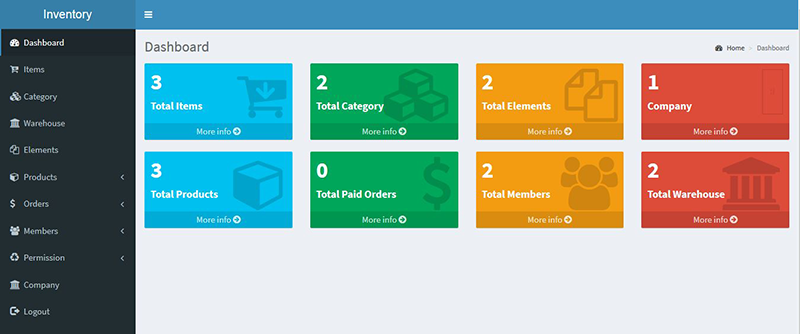
\includegraphics[width=1\textwidth]{simillar_systems/dineth1.png}
	\caption{Dashboard of the Sales and Inventory Management System in Dineth Stores}
\end{figure}

\subsection{Sales management system in Shaanthi Grocery}

This grocery uses their sales management system to perform daily transactions and keep track of history regarding sales.  Furthermore, it has facilities to keep track of the inventory, manage purchase orders and manage purchase returns.

\begin{figure}[H]
	\centering
	\includegraphics[width=1\textwidth]{simillar_systems/shaanthi1.png}
	\caption{Item Management Window of the Sales Management System in Shaanthi Grocery}
\end{figure}

\begin{figure}[H]
	\centering
	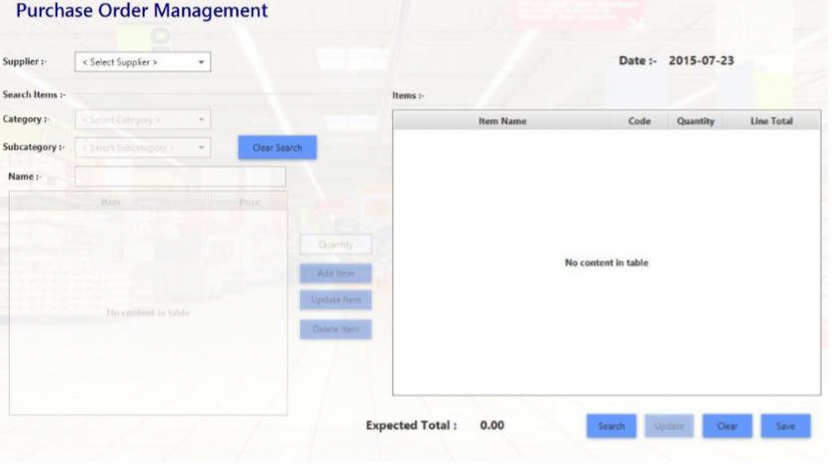
\includegraphics[width=1\textwidth]{simillar_systems/shaanthi2.png}
	\caption{Purchase Order Window of the Sales Management System in Shaanthi Grocery}
\end{figure}

\subsection{Comparison between similar systems}
\begin{table}[H]
	\centering
	\begin{tabular}{ |c|c|c| }
		\hline
		\bf{Features}             & \bf{CBIS in Dineth Stores} & \bf{CBIS in Shaanthi Grocery} \\
		\hline
		Item and Supplier Details & Yes                        & Yes                           \\
		\hline
		Employee Details          & Yes                        & No                            \\
		\hline
		Purchase Orders           & Yes                        & Yes                           \\
		\hline
		Manage Sales              & Yes                        & Yes                           \\
		\hline
		Payments and Receipts     & Yes                        & Yes                           \\
		\hline
		\acrshort{grn} Management & Yes                        & Yes                           \\
		\hline
		Generate reports          & Yes                        & Yes                           \\
		\hline
		Notifications reports     & Yes                        & No                            \\
		\hline
	\end{tabular}
	\caption{Comparison between similar systems}
\end{table}

\section{Existing System}
Current system with a file-based approach stores all of the records in physical papers. Due to this procedure it takes a long time to process transactions. Since this organization deals with huge amount of data, manipulation and retrieval of existing records has become very inefficient.

Furthermore, when new sales are made or customer payment accepted, inventory and payment details need to be manually updated in multiple places. When issuing purchase orders, accepting \acrshort{grn}s and ordering supplies there is a great deal of paperwork that needs to be done. Also, management have difficulties finding  necessary reports and data due the large amount of unorganized paperwork. Following figure briefly shows the existing manual system.

\begin{figure}[H]
	\centering
	\includegraphics[width=\textwidth]{uml/usecase_manual.jpg}
	\caption{Use Case Diagram of the current manual system}
\end{figure}

\section{Analysis of the requirements}

\subsection{Requirement gathering techniques}
In order to capture functional and non-function requirements of the existing system, following techniques were used.

\begin{itemize}
	\item Observation
	\item Document Analysis
	\item Interviews
\end{itemize}

\subsection{Functional Requirements}
Functional requirements specify features developers must implement in order to allow users to accomplish their tasks (user requirements).  These should describe business requirements end-users are expecting. Following are the list of functional requirements found in this system.

\begin{itemize}
	\item Manage item details
	\item Manage customer details.
	\item Manage employee details.
	\item Manage purchase order details.
	\item Manage \acrshort{grn}s.
	\item Manage material details.
	\item Manage product details.
	\item Manage users.
	\item Manage roles.
	\item Manage role privileges.
	\item Generate reports.
	\item Generate bills.
\end{itemize}

\subsection{Non-Functional Requirements}
Non-functional requirements describe the features this system should have. Non-functional requirements are difficult to work with than functional ones because they depends on each user perspective and their preferences. But, user friendliness of the system depends on how well these non-functional requirements are met.  Following are the list of non-functional requirements aim to offer in the proposed system.

\begin{itemize}
	\item {\bf{Security}}\\
	      Since system will store sensitive details such as personal employee details, there are security measures in place such as user access management, privileges control and unauthorized accedes prevention.

	\item {\bf{Usability}}\\
	      System user-interface contain easy to to navigate menus, dashboard and a clear way to indicate the current location user is in. This maximizes the usability of the system allowing user to switch between modules seamlessly.

	\item {\bf{Accuracy}}\\
	      Proposed system has mechanisms in place to to handle transactions with minimum error probability allowing users to perform their tasks and retrieve information with high accuracy.

	\item {\bf{User friendliness}}\\
	      User-interface of the system is very simple and easy to to navigate allowing even a new user to learn to perform tasks very quickly.

	\item {\bf{Efficiency and consistency}}\\
	      System has very fast response rates and accurate database management mechanisms preventing issues such as data inconsistencies and slow data retrieval.
\end{itemize}

\section{Process model}
Due to the nature of requirements of this system, iterative and incremental approach was selected as the development methodology. The most prominent reason for this was unclear nature of requirements and the complexity of operations in the existing manual system.

Furthermore, actors involved in this system have a tendency of requesting changes to existing requirements and difficulty in explaining existing business processes. This also influenced selecting this methodology because it allows us to have a flexible way to manage changes even in a later stage of the development.

\"In an Iterative Incremental model, initially, a partial implementation of a total system is constructed so that it will be in a deliverable state. Increased functionality is added. Defects, if any, from the prior delivery are fixed and the working product is delivered. The process is repeated until the entire product development is completed. The repetitions of these processes are called iterations. At the end of every iteration, a product increment is delivered. \cite{point_2019_sdlc}\".

As stated above, this modal provide a flexible framework for developing the system with continuous user-feedback and ability to modify existing features even in a later stage of the development.

If a modal like waterfall were to use for this system, it would be very difficult or sometimes impossible to cater to client's requests. Also, since requirements should be clear and entire system design should be completed early in waterfall, end-product could potentially fail to match client expectations. Thus, choosing iterative and incremental modal as the development methodology for this project allows to overcome the difficulties that could have occurred in a strict modal.

\begin{figure}[H]
	\centering
	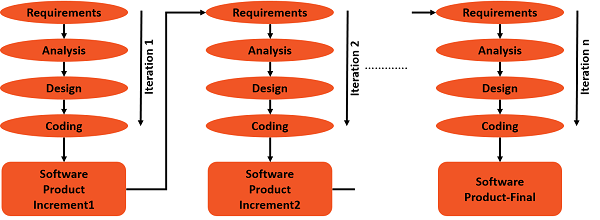
\includegraphics[width=\textwidth]{iterative_incremental_model.png}
	\caption{Iterative and Incremental Model}
\end{figure}

\subsection{Steps in Iterative and Incremental Model}
\begin{itemize}
	\item Requirement analysis
	\item Design
	\item Coding
	\item Testing
	\item Next iteration
\end{itemize}

\newpage
\chapter{Design}
After performing the analysis phase, designing phase should be performed to provide a technical solution for gathered functional and non-functional requirements during the analysis phase. This design, or rather solution will serve as the foundation in later stages such as coding and implementation.

In this chapter alternative solutions and design diagrams will be explained with the help of \acrshort{uml}. Furthermore, chosen architectural design and user interface design strategeis of the system will also be explained in detail.

\section{Design strategies}

\subsection{Maintain new system for some processes alongside existing file-based system}
With this strategy new system could have been developed to support the existing processes and only to provide features such as report generation and billing. But, this will result in loss of time and cost due to reasons such as wastage of papers and manpower.

\subsection{Use an existing free production management software}
Even though there exists software targeted towards production management, they are mostly developed for generalized businesses processes. Since this organization have unique business processes and specific requirements, usage of that sort of software could have done more harm than good. Furthermore, there is no way to guarantee the reliability of freely available solutions.

\section{Justification for the selected design strategy}
This is system is being developed as a web-based solution since owners and management of this organization is hoping to accesses information such as reports outside of the workplace. Furthermore, since their manages sometimes interact with clients and suppliers outside, it’s required for them to being able to access the system via internet.

Beside above requirements, there are several benefits using a web-based solution for this organization.

\begin{itemize}
	\item Reduced cost for hardware and infrastructure.

	\item Platform independent nature of web-based solutions (Since only real requirements are a web browser and internet access).

	\item Ability to access the system even outside of work premises. This can be considered as the most important benefit.
\end{itemize}

\section{Architectural design}
This proposed system is being implemented using the \acrshort{mvc} or \acrlong{mvc} structural design. This pattern isolates the representation of information from user interactions. This is a widely used Object-Oriented design pattern for developing web-based and desktop applications.

Since this model provides an isolation between different components based on their  usage, it’s very suitable for the development of this solution. Furthermore, nature of this model allows developers to focus on important parts of the system without getting distracted by unnecessary details. This model consists of the following three major components.

\begin{itemize}
	\item {\bf{Model}}\\
	      This represents the shape of the data and business logic. It maintains the data of the application. Models are being used as objects to retrieve and store information to and from a database.

	\item {\bf{View}}\\
	      This is a user interface. View display data with the help models to the user and also enables them to modify the data.

	\item {\bf{Controller}}\\
	      This handles user requests and logical operations. Typically, the user interacts with a View, which in-turn raises appropriate URL request, this request will be handled by a controller.
\end{itemize}

\begin{figure}[H]
	\centering
	\includegraphics[width=0.5\textwidth]{mvc_architecture.png}
	\caption{\acrshort{mvc} Architecture}
\end{figure}

\acrshort{mvc} modal is popular due to it’s powerful nature of separating data and its representations. Simply put, same data can be shown to two different users in two different ways with the help of this modal.

When modeling system operations and business processes \acrshort{uml} Diagrams were used. \acrshort{uml} is a set of modeling diagrams which allows to look at a system in multiple angles. Graphical symbols provided by \acrshort{uml} allows to modal the proposed system in a way that can improve the understandability between designers and developers, sometimes end-users.

Among various diagrams described in the \acrshort{uml} specification, following were used to model this proposed system.

\begin{itemize}
	\item Use case diagram
	\item Activity diagram
	\item Class diagram
	\item Sequence diagram
\end{itemize}

\newpage
\subsection{Use Case Diagram}
A use case diagram is a dynamic or behavior diagram in \acrshort{uml}. Use case diagrams model the functionality of a system using actors and use cases. Use cases are a set of actions, services, and functions that the system needs to perform \cite{paradigm_2018_uml}.

In this context, a \"system\" is something being developed or operated, such as a web site. The \"actors\" are people or entities operating under defined roles within the system.

\begin{figure}[H]
	\centering
	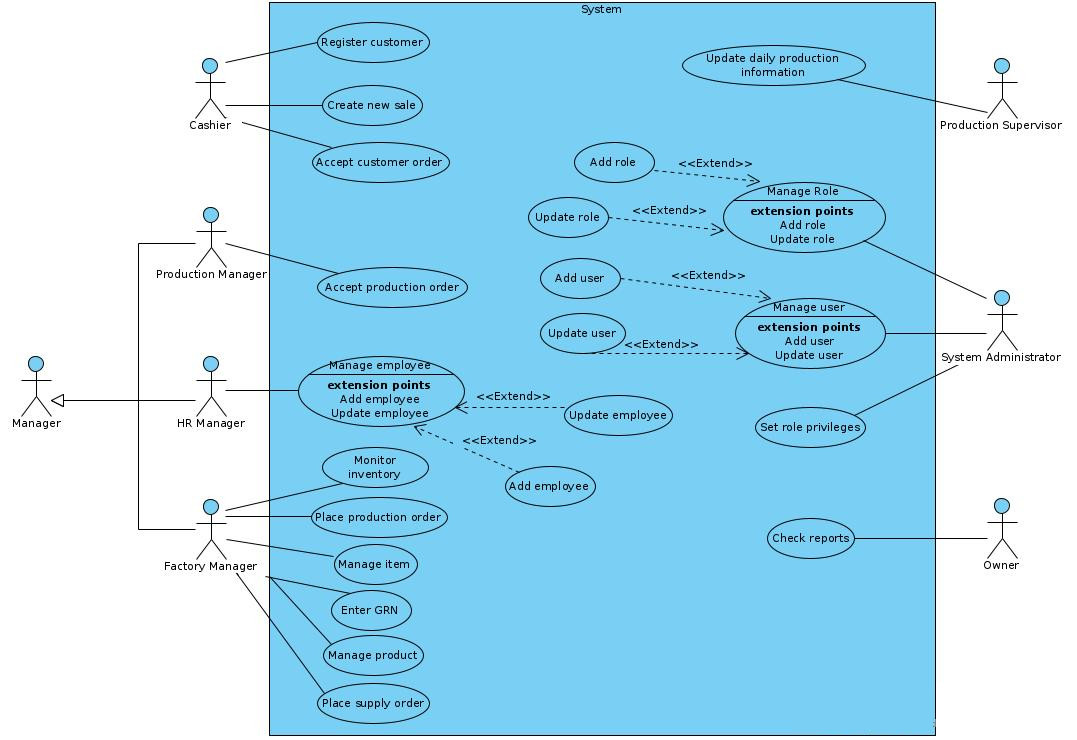
\includegraphics[width=\textwidth]{uml/usecase_system.png}
	\caption{Use Case Diagram for the entire system}
\end{figure}

\newpage
\subsection{Use Case Narratives}

\begin{table}[H]
	\centering
	\begin{tabular}{ |c|p{10.2cm}| }
		\hline
		Use Case        & Create new production order    \newline                               \\
		\hline
		Actor/s         & Factory Manager  \newline                                             \\
		\hline
		Description     & Create new production order based on inventory status  \newline       \\
		\hline
		Preconditions   &
		1. User mused be logged in. \newline
		2. User should have access to production order view. \newline
		3. Production order view must be opened. \newline
		4. Before submission relevant production details should be added.\newline
		\\
		\hline
		Post-conditions &
		1. Production order added to the system and visible to the production manager. \newline \\
		\hline
		Flow of events  &
		1. Select relevant items.\newline
		2. Select their quantities.\newline
		3. Click “Add” button.\newline
		\\
		\hline
		Alternatives    &
		1. User gets a permission error due to lack of privileges. \newline
		\\
		\hline
	\end{tabular}
	\caption{Use Case Narrative for creating a production order}
\end{table}

\begin{table}[H]
	\centering
	\begin{tabular}{ |c|p{10.2cm}| }
		\hline
		Use Case        & Login to the sysem    \newline            \\
		\hline
		Actor/s         & All Actors  \newline                      \\
		\hline
		Description     & User log in to the system  \newline       \\
		\hline
		Preconditions   &
		1. User account must be present. \newline
		2. Username and password must be correct. \newline
		\\
		\hline
		Post-conditions &
		1. Appropriate dashboard is displayed to the user. \newline \\
		\hline
		Flow of events  &
		1. User enter username and password.\newline
		2. System validate and check user details.\newline
		3. User get redirected to the dashboard.\newline
		\\
		\hline
		Alternatives    &
		1. Error message getting displayed due to invalid credentials. \newline
		\\
		\hline
	\end{tabular}
	\caption{Use Case Narrative for logging in to the the system}
\end{table}

\newpage
\subsection{Activity Diagram}
Activity diagram is another important behavioral diagram in \acrshort{uml} diagram to describe dynamic aspects of the system. Activity diagram is essentially an advanced version of flow chart that modeling the flow from one activity to another activity \cite{paradigm_2018_uml}.

\begin{figure}[H]
	\centering
	\includegraphics[width=\textwidth]{uml/activity_production_order.jpg}
	\caption{Activity Diagram for a production order}
\end{figure}

\begin{figure}[H]
	\centering
	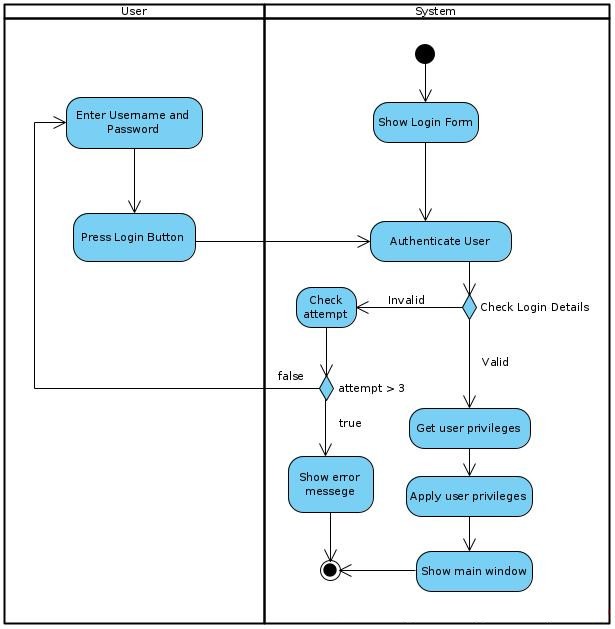
\includegraphics[width=\textwidth]{uml/activity_login.jpg}
	\caption{Activity Diagram for logging into the system}
\end{figure}

\newpage
\subsection{Class Diagram}
In software engineering, a class diagram in the \acrfull{uml} is a type of static structure diagram that describes the structure of a system by showing the system's classes, their attributes, operations (or methods), and the relationships among objects \cite{paradigm_2018_uml}.

\begin{figure}[H]
	\centering
	\includegraphics[width=\textwidth]{uml/class_system.jpg}
	\caption{Class Diagram for the entire system}
\end{figure}

\newpage
\subsection{Sequence Diagram}
\acrshort{uml} Sequence Diagrams are interaction diagrams that detail how operations are carried out. They capture the interaction between objects in the context of a collaboration. Sequence Diagrams are time focus and they show the order of the interaction visually by using the vertical axis of the diagram to represent time what messages are sent and when \cite{paradigm_2018_uml}.

\begin{figure}[H]
	\centering
	\includegraphics[width=\textwidth]{uml/sequence_production_order.jpg}
	\caption{Sequeunce Diagram for a production order}
\end{figure}

\newpage
\subsection{Data modeling}
Include description about data modeling and ER diagrams.
Include 5 or more ER diagram segments of the system.

\subsection{User interface design}
Include description about UI designing and UI Wireframing.
Include 5 or more Wireframes of the system.

%>>>>>>>>>>>>>>>>>>>>> End of Thesis 

%-------- Bibliography
%\newpage
\singlespacing
\printbibliography[title={References}]
\end{document}